\subsection{Definition of the $\chi$ Field}
  \label{subsec:definition-of-the-chi-field}

  We postulate the existence of a single fundamental scalar quantity, denoted $\chi$, which constitutes the primitive
  substrate of physical reality.
  The field $\chi$ is not defined on a pre-existing spacetime manifold and does not presuppose any metric, causal, or
  geometric structure.
  Instead, spacetime itself emerges as an effective description of the relational and dynamical properties of
  $\chi$ configurations.

  Ontologically, $\chi$ is a real scalar order parameter whose value characterizes the local geometric state of the
  underlying substrate.
  It carries dimensions of length and encodes a characteristic wavelength associated with physical processes.
  This wavelength does not evolve \textit{in} time; rather, its monotonic and irreversible relaxation defines what is
  operationally perceived as the flow of time.

  Temporal ordering emerges from the global, monotonic evolution of $\chi$ across physical processes,
  establishing an intrinsic arrow of time without reference to an external temporal coordinate.
  Spatial separation, in turn, arises from relational differences between $\chi$ values across configurations,
  giving rise to an effective notion of distance once a stable geometric regime is established.
  In this sense, time corresponds to ordering, while space corresponds to relational structure.

  At no stage is $\chi$ interpreted as a spacetime coordinate or as a material field propagating on spacetime.
  Rather, spacetime coordinates and metric structure appear as secondary, coarse-grained constructs that become
  meaningful only when $\chi$ configurations admit a quasi-stable geometric interpretation.
  The spacetime metric thus functions as an emergent, effective descriptor of resistance to $\chi$
  relaxation\footnote{The term ``relaxation'' is used here in a geometric and dynamical sense, and should not be
confused with thermodynamic relaxation processes involving dissipation or entropy increase.} and of the propagation of perturbations within the field.

  This role of $\chi$ is analogous to that of thermodynamic order parameters such as temperature:
  it encodes collective geometric information about an underlying substrate without being itself a fundamental
  spacetime entity.
  In the Cosmochrony framework, $\chi$ therefore provides the minimal ontological basis from which time, space,
  gravitation, and quantum phenomena jointly emerge.

  In the following sections, spacetime coordinates and metric quantities will be introduced as effective tools,
  valid in regimes where $\chi$ admits a stable geometric interpretation.

  \begin{figure}[h]
    \centering
    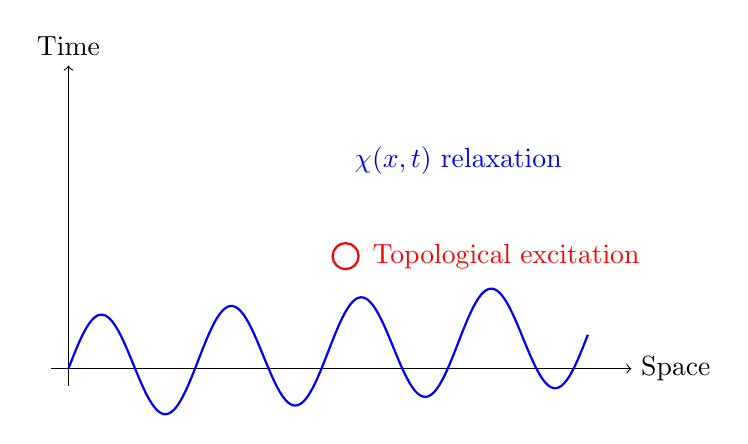
\begin{tikzpicture}[scale=1.1]

% Axes
      \draw[->] (-0.2,0) -- (6.5,0) node[right]{Space};
      \draw[->] (0,-0.2) -- (0,3.5) node[above]{Time};

% Wave
      \draw[thick, blue, domain=0:6, samples=200]
      plot (\x,{0.6*sin(2*pi*\x/1.5 r) + 0.4*\x/6});

% Particle crest
      \draw[red, thick] (3.2,1.3) circle (0.15);
      \node[red, right] at (3.4,1.3) {Topological excitation};

% Annotation
      \node[blue] at (4.5,2.4) {$\chi(x,t)$ relaxation};

    \end{tikzpicture}
    \caption{Conceptual representation of Cosmochrony. A single continuous wave field $\chi(x,t)$
      undergoes irreversible relaxation,
      characterized by a monotonic increase of its characteristic wavelength. Localized topological excitations
      correspond to particles.}
    \label{fig:chi_concept}
  \end{figure}

  \paragraph{On the use of spacetime language.}
    Throughout this work, phrases such as ``spacetime coordinates,'' ``metric tensor,'' and ``four-dimensional manifold'' appear frequently.
    These should be understood as \emph{emergent effective descriptions} valid in regimes where $\chi$ has relaxed into a quasi-stable geometric configuration.
    They are not fundamental ingredients of the theory.

    At the deepest level, only $\chi$ and its local variation structure exist.
    The appearance of familiar geometric language reflects the effectiveness of spacetime as a coarse-grained description of collective $\chi$ behavior, analogous to how thermodynamic variables (temperature, pressure) emerge from molecular dynamics without those variables being fundamental.

    This interpretational stance is essential for distinguishing Cosmochrony from approaches that merely reformulate existing geometric theories in different variables.
